\documentclass[../interim.tex]{subfiles}


\begin{document}


\chapter{Background}

This section introduces some technical background which will likely be required as part of the project. It includes an introduction to neural networks and CNNs, a comparison of some existing object tracking and object detection algorithms and a discussion on knowledge representation and reasoning and symbolic rule learning.

\section{Deep Learning}

Deep neural networks (DNNs) have emerged as a very successful algorithm for machine learning; deep learning has been used to beat records in tasks such as image recognition, speech recognition and language translation~\cite{deep-learning-intro}. Many different architectures have been proposed to solve various tasks, these architectures include convolutional neural networks (CNNs), which are designed to process data that come in the form of multiple arrays~\cite{deep-learning-intro}, and recurrent neural networks (RNNs), which are designed to process sequences of arbitrary length~\cite{def:rnn}. The following section gives a brief introduction to CNNs and describes some of their use cases.

\subsection{Convolutional Neural Networks}

CNNs contain three types of layers: convolution, pooling and fully connected. Units (artificial neurons) in a convolution layer are organised into feature maps. The inputs to each unit in a feature map come from the outputs of the units in a small region of the previous layer, the output of the unit is then calculated by passing the weighted sum of its inputs through an activation function such as ReLU. The set of weights, also known as a filter or kernel, is the part of the layer which is learned through backpropagation. Every unit in a feature map has the same kernel. Each feature map in a layer has its own kernel. Pooling layers reduce the size of the input by merging multiple units into one. A typical pooling operation is max-pooling, which computes the maximum of a local patch of units. Finally, in fully-connected layers (which are typically placed at the output of the CNN) every unit in a layer is connected to every unit in the previous layer. An example CNN architecture is shown in figure~\ref{fig:example-cnn}.

\begin{figure}
  \centering
  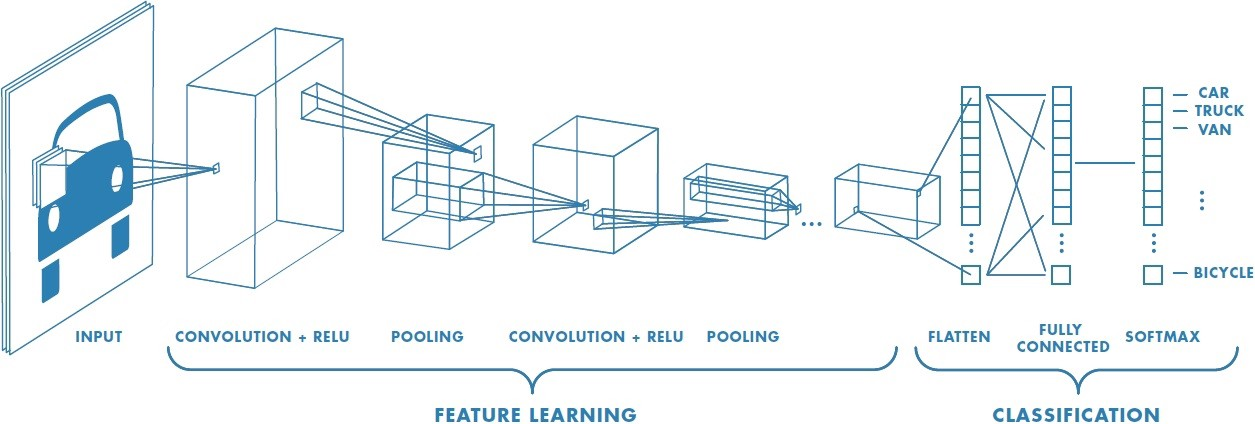
\includegraphics[width=0.8\textwidth]{cnn-example.jpg}
  \caption{An example of a CNN architecture. The input image is passed through a series of convolution and pooling layers before being flattened into a one-dimensional layer and passed through one final fully connected layer. The softmax classification function is then applied at the output.}
  \label{fig:example-cnn}
\end{figure}

CNNs have proven to be adept at a number of tasks involving images, including image classification~\cite{cnn-uses:classification} and object detection~\cite{cnn-uses:yolo-v3, cnn-uses:faster-r-cnn}. We explore these further in Section~\ref{section:image-proc}.


\section{Image Processing}
\label{section:image-proc}

\subsection{Object Detection}

The object detection task could formally be defined as designing a model which, when given an image, can produce a rough localisation of objects of interest in the image (in the form of a bounding box) and classify eac of these objects into a set of predefined classes. In this section we introduce two well known object detection algorithms, Faster R-CNN~\cite{cnn-uses:faster-r-cnn} and You Only Look Once (YOLO)~\cite{cnn-uses:yolo-v3}.

Faster R-CNN is an evolution of previous object detection algorithms, R-CNN~\cite{r-cnn} and Fast R-CNN~\cite{fast-r-cnn}. Faster R-CNN builds on its predecessors by adding a region proposal network (RPN) - a neural network which takes an image and produces a set of region of interest (RoI) proposals. This method of region proposal is much faster than previous algorithms (such as those used in~\cite{r-cnn} and~\cite{fast-r-cnn}) since it is able to make use of the GPU, as opposed to requiring the CPU. Faster R-CNN then uses a similar classifier and bounding box regressor as Fast R-CNN at the output; this section of the network also receives the feature maps from the final layer of the RPN, in this sense the initial layers of the network are shared between the region proposal section and the classifier/regressor section. A diagram of the Faster R-CNN architecture is shown in figure~\ref{fig:fasterrcnn}.

\begin{figure}
  \begin{subfigure}{0.4\textwidth}
    \centering
    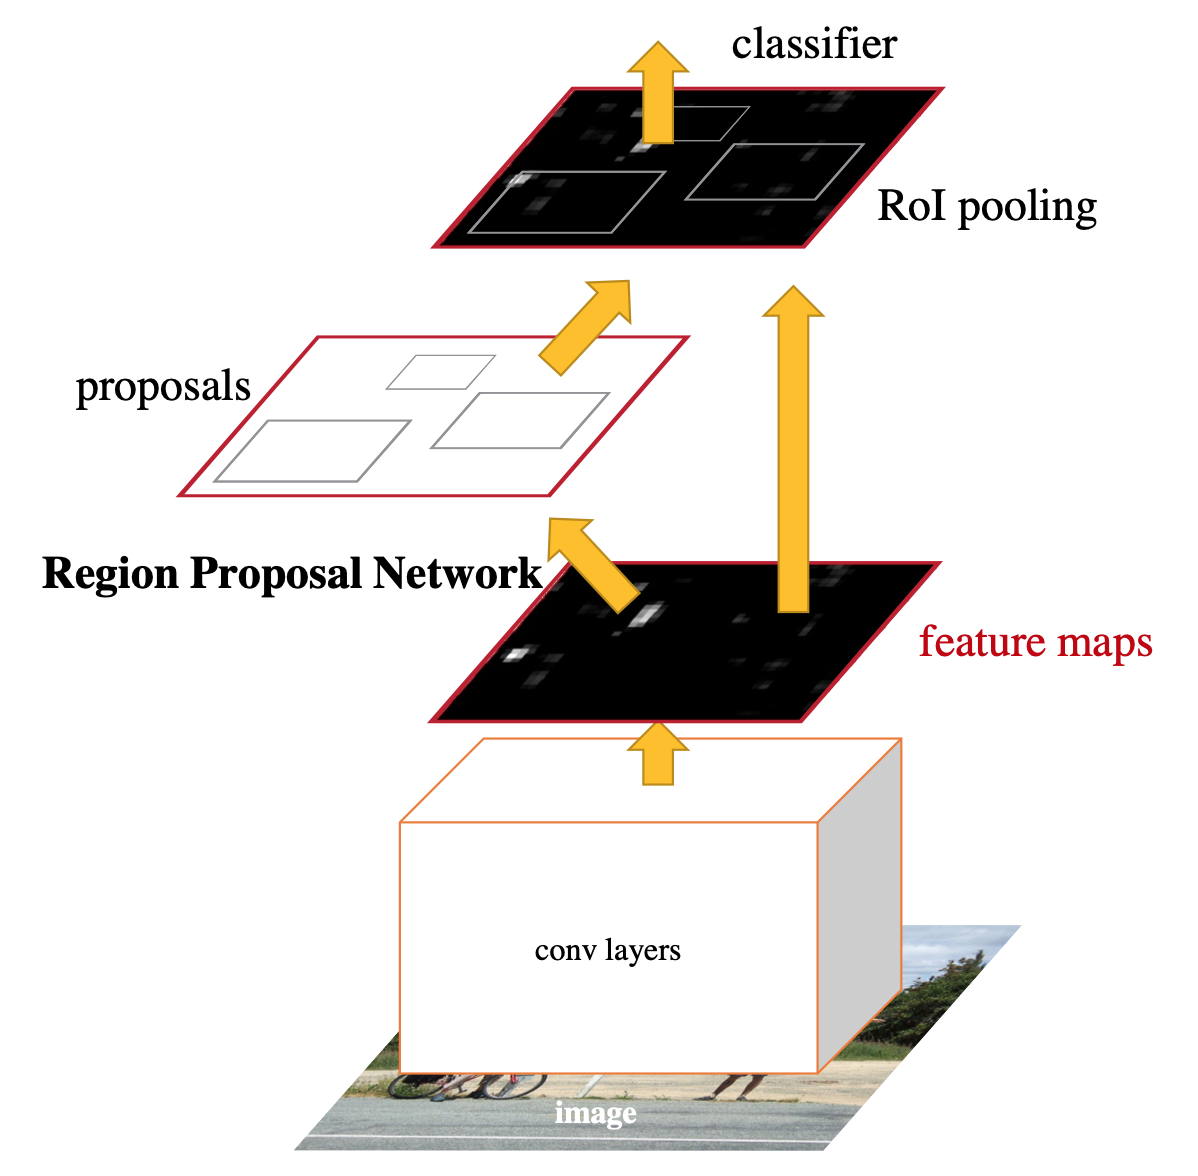
\includegraphics[width=\textwidth]{faster-r-cnn.png}
    \caption{Diagram of the Faster R-CNN architecture. Figure from~\cite{cnn-uses:faster-r-cnn}.}
    \label{fig:fasterrcnn}
  \end{subfigure}
  \hfill
  \begin{subfigure}{0.55\textwidth}
    \centering
    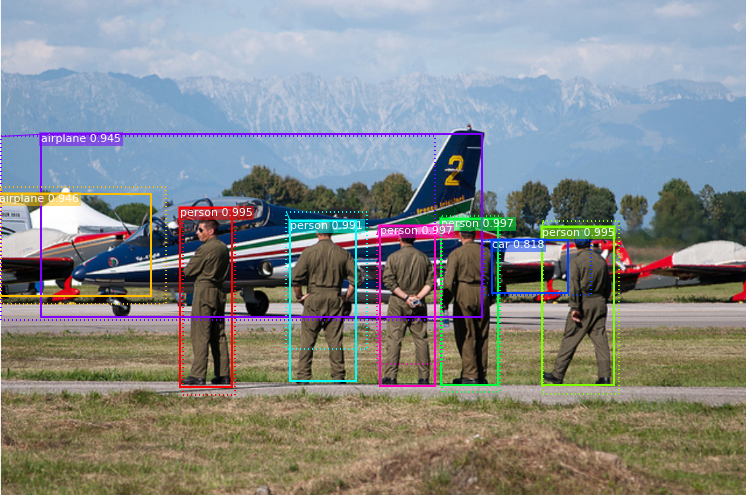
\includegraphics[width=\textwidth]{bounding-boxes.png}
    \caption{An example of the bounding boxes and confidence scores produced by an object detection algorithm. Image from~\cite{obj-detection-examples}.}
    \label{fig:bounding-boxes}
  \end{subfigure}
  \caption{ }
\end{figure}

The three object detection algorithms mentioned above all work by first producing region proposals, then producing a more accurate localisation and a score for each region and finally removing any low-scoring or redundant regions. This requires the algorithm to `look' at the image multiple times (around 2000 times for R-CNN). You Only Look Once (YOLO) is a significantly more time-efficient algorithm which, as the name suggests, takes a single look at the image. A convolutional neural network is used to simultaneously predict multiple bounding boxes and the class probabilities for each box. As well as being very fast, YOLO makes fewer than half the number of background errors (where the algorithm mistakes background patches for objects) as Fast R-CNN~\cite{yolo}. YOLO is, however, slightly less accurate than some of the slower methods for object detection~\cite{cnn-uses:yolo-v3}.

\subsection{Commonly Used Metrics}

In this section we present some commonly used metrics for classification and object detection tasks. We use TP, TN, FP and FN to mean True Positive, True Negative, False Positive and False Negative, respectively.

Firstly, for classification tasks the following terminology is commonly used:
\begin{itemize}
  \item $Accuracy = \frac{TP + TN}{TP + TN + FP + FN}$. The accuracy is the ratio of correct predictions to the total number of predictions.

  \item $Precision = \frac{TP}{TP + FP}$. The precision is the ability of a classifier to not label the negative data as positive.

  \item $Recall = \frac{TP}{TP + FN}$. The recall is the ability of the classifier to find the positively-labelled data.

  \item $F_1 = 2 * \frac{precision * recall}{precision + recall}$. The $F_1$ score is a way of combining the precision and recall scores.
\end{itemize}

Each object detector model will output a confidence score for each object classification it makes. We can then set a threshold value which determines what is counted as a classification of an object. Altering this threshold value will give different precision and recall values for the model, which can then be plotted on a precision-recall graph. Example precision-recall curves are shown in figure~\ref{fig:prec-recall}.

\begin{figure}
  \centering
  \begin{subfigure}{0.48\textwidth}
    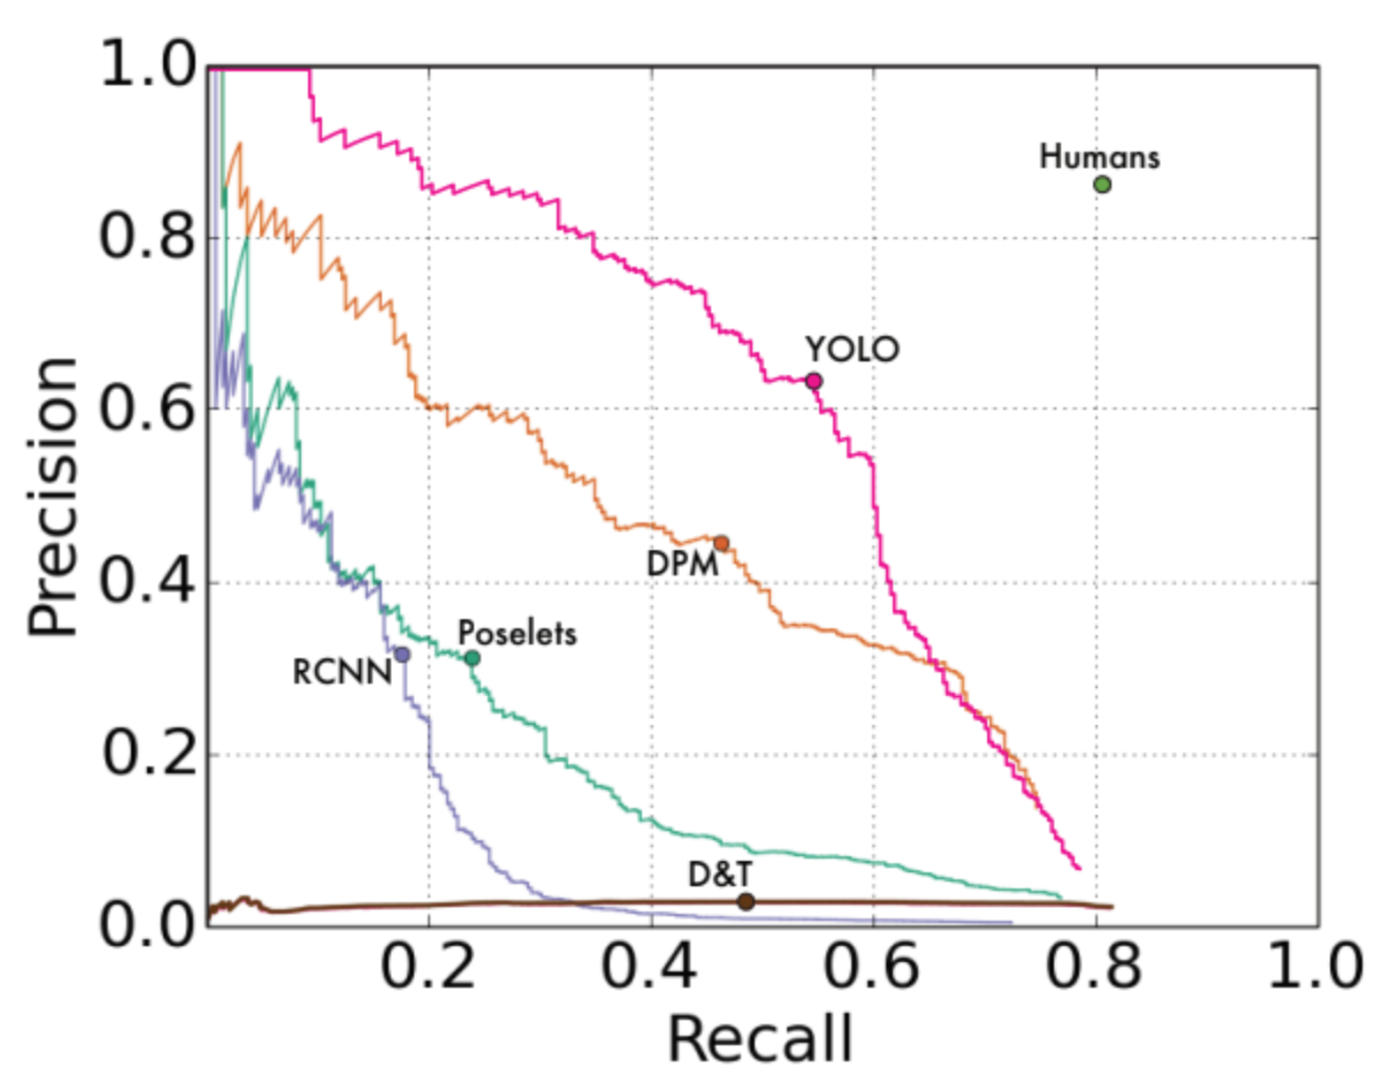
\includegraphics[width=\textwidth]{prec-recall.png}
    \caption{Example precision-recall curves for various object detection models. Image from~\cite{yolo}.}
    \label{fig:prec-recall}
  \end{subfigure}
  \hfill
  \begin{subfigure}{0.48\textwidth}
    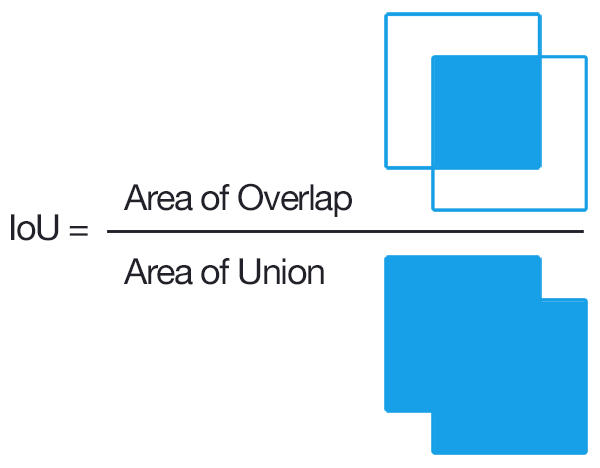
\includegraphics[width=\textwidth]{iou-image.png}
    \caption{Visual explanation of the intersection over union metric. Image from~\cite{iou-image}.}
    \label{fig:iou}
  \end{subfigure}
  \caption{Precision-recall curves and definition of intersection over union}
\end{figure}

For object detection tasks, where a bounding box is produced as a rough localisation of an object's position, metrics which measure the accuracy of the localisation of an object are required. One very common metric is the Average Precision (AP), which is roughly defined as the area under the precision-recall curve (estimates of this value are usually used for competition datasets). In order to assess how well a model localises an object in an image the Interesection over Union (IoU) metric is commonly used. Figure~\ref{fig:iou} gives a visualisation on how IoU is calculated. Each IoU threshold will produce its own precision-recall curve.


\subsection{Multiple Object Tracking}

Multiple Object Tracking (MOT) is a computer vision task that aims to identify and track objects from a sequence of images without any prior knowledge about the appearance or number of targets~\cite{obj-tracking-survey}. Most object tracking methods share a very similar pipeline~\cite{obj-tracking-survey}, as follows:
\begin{itemize}
  \item \textbf{Detection}. Each input frame is analysed to identify objects using bounding boxes.

  \item \textbf{Feature Extraction}. Algorithms extract appearance, motion and/or interaction features from objects.

  \item \textbf{Affinity Computation}. Features are used to compute a similarity score between objects.

  \item \textbf{Association}. Similarity scores are used to associate detections and compute the object trajectories.
\end{itemize}

The Simple Online and Realtime Tracking (SORT)~\cite{sort-obj-tracking} algorithm is one of the best performers~\cite{obj-tracking-survey}. It makes use of Faster R-CNN for object detection, the Kalman filter~\cite{kalman-filter} framework for predicting object motion, IoU as a similarity function and the Hungarian algorithm~\cite{hungarian-algo} for association. SORT attempts to track objects using motion prediction, other algorithms, however, focus on extracting features from objects, such as Histogram of Orientated Gradients (HOG)~\cite{hog-features} features, and using these to match objects in successor frames. More recent methods tend to use features extracted directly from a CNN.


\section{Knowledge Representation and Reasoning}

Knowledge Representation and Reasoning (KRR) is concerned with how intelligent agents store and manipulate their knowledge. In this section we discuss Answer Set Programming, a logic programming framework, action languages, which can be used to define the behaviour of a system, and methods for learning logical rules inductively.

\subsection{Answer Set Programming}

Answer Set Programming (ASP) is a form of declarative logic programming that can be used to solve difficult search problems. Whereas imperative programs define an algorithm for finding a solution to a problem, logic programs simply define a problem, it is then the job of logic program solvers to find a solution to the problem. ASP also differs from Prolog, another popular logic programming language, in that ASP programs are purely declarative. This means that reordering rules or atoms within rules has no effect on the output of the solver~\cite{asp-primer}. ASP solvers work by finding the answer sets of the program, where each rule in the program imposes restrictions on what can be an answer set. An answer set can be thought of as a set of ground atoms which satisfies every rule of the program (although the full definition of an answer set is too in-depth for this discussion).

The following templates are a some of the possible forms of rules in an ASP program:
\begin{align}
  a \text{ :- }& b_1, ..., b_k, not \text{ } b_{k+1}, ..., not \text{ } b_m. \label{asp-rule:normal}\\
  \{c_1;...;c_n\} \text{ :- }& b_1,...,b_k, not \text{ } b_{k+1}, ..., not \text{ } b_m. \label{asp-rule:choice}\\
  \text{:- }& b_1,...,b_k, not \text{ } b_{k+1}, ..., not \text{ } b_m. \label{asp-rule:constraint}
\end{align}

Where each $a$, $b_i$ and $c_i$ are atoms in first-order logic. The left hand side of the rule is known as the head, and the right hand side is known as the body. The $not$ in the rule body stands for negation-as-failure, which means that $not$ $b_i$ will be satisfied when $b_i$ cannot be proved. Each rule requires that when the body is satisfied - that is, when every member of the body is satisfied - the head must be satisfied. Rule~\ref{asp-rule:choice} is known as a choice rule. The head of a choice rule can be satisfied by any subset of the atoms inside the brackets (including the empty set); in effect, a choice rule creates possible answer sets. Finally, rule~\ref{asp-rule:constraint} is known as a constraint. The body of a constraint must not be satisfied; intuitively, a constraint rules out answer sets.

As well as negation as failure, ASP also has a notion of `strong negation'. The strong negation of an atom $p$ is written $\neg p$. Strong negation can be thought of as logical negation, although it does not always have the same properties. In practice, ASP solvers implement strong negation by treating $\neg p$ as an additional atom, and enforce that no answer set can contain both $p$ and $\neg p$.

\subsection{The Action Language $\mathcal{AL}$}

Action languages are formal models for describing the behaviour of dynamic systems. In this section we present the version of $\mathcal{AL}$ given in~\cite{krr-asp-book}. $\mathcal{AL}$'s signature contains three special sorts: \textit{statics}, \textit{fluents} and \textit{actions}. Fluents are partitioned into two sorts: \textit{inertial} and \textit{defined}. Statics and fluents are both referred to as `domain properties'. A `domain literal' is a domain property or its negation. Statements in $\mathcal{AL}$ can be of the following form:
\begin{gather}
  a \textbf{ causes } l_{in} \textbf{ if } p_0,...,p_m \label{al:causal} \\
  l \textbf{ if } p_0,...,p_m \label{al:constraint} \\
  \textbf{impossible } a_0,...,a_k \textbf{ if } p_0,...,p_m \label{al:exec}
\end{gather}

Where $a$ is an action, $l$ and $p_0,...,p_m$ are domain literals and $l_{in}$ is a literal formed by an inertial fluent. Statement~\ref{al:causal} is known as a \textit{causal law}, \ref{al:constraint} as a \textit{state constraint} and \ref{al:exec} as an \textit{executability condition}. A collection of $\mathcal{AL}$ statements is known as a `system decription'. An $\mathcal{AL}$ system description can be used to model the behaviour of dynamic systems with discrete states; each state can be seen as the set of fluents which are true and transitions between states are caused by actions.

It also possible to encode a given $\mathcal{AL}$ system description, along with a number of `domain-independent' axioms, in ASP. The method for creating this encoding is given in Appendix~\ref{appendix-al}.

\subsection{Symbolic Rule Learning}

Inductive Logic Programming~\cite{ilp-intro} (ILP) is a field of symbolic AI research concerned with learning symbolic rules which, when combined with background knowledge, entail a set of positive examples and do not entail any negative examples. ILASP~\cite{ilasp-system} (Inductive Learning of Answer Set Programs) is an ILP framework for learning ASP programs.

The authors of~\cite{ilasp-1} define the \textit{Learning from Answer Sets} ($ILP_{LAS}$) task (which is the task solved by the original version of ILASP), by first defining a \textit{partial interpretation}. A partial interpretation $E$ is a pair of sets of atoms $E^{inc}$ and $E^{exc}$, known as the \textit{inclusions} and \textit{exclusions} of $E$. An answer set $A$ \textit{extends} $E$ if it contains all of the inclusions ($E^{inc} \subseteq A$) and none of the exlusions ($E^{exc} \cap A = \emptyset$). An $ILP_{LAS}$ task is then defined as the tuple $T = \langle B, S_M, E^+, E^- \rangle$, where $B$ is the background knowledge, $S_M$ is the search space, $E^+$ and $E^-$ are the partial interpretations for the positive and negative examples, respectively. An hypothesis $H$ is known as an inductive solution of $T$ if and only if all of the following are true:
\begin{enumerate}
  \item $H \subseteq S_M$
  \item $\forall e^+ \in E^+ \text{ } \exists A \in AS(B \cup H) \textit{ such that } A \textit{ extends } e^+$
  \item $\forall e^- \in E^- \text{ } \nexists A \in AS(B \cup H) \textit{ such that } A \textit{ extends } e^-$
\end{enumerate}

\noindent
Where $AS(P)$ refers to the answer sets of a program $P$.

\vspace{3mm}
Later versions of ILASP are capable of solving more complex tasks, including learning weak constraints~\cite{ilasp-wc} (a method for specifying preferences in ASP), learning from context dependent examples~\cite{ilasp-cde} and learning from noisy examples~\cite{ilasp-noisy}.

\end{document}
